\documentclass [a4paper,11pt,twoside,notitlepage,openright]{report} %print on both side
\usepackage[bookmarks=false, colorlinks=false,unicode]{hyperref}
%\usepackage[abbr,dcucite]{harvard}      %style ofliterature
\usepackage{Styles/Skripta}
\usepackage{Styles/Diplomka}
\usepackage{Styles/Colors}
\usepackage{url}
\usepackage{graphicx}
\usepackage{epstopdf}

%------<<<<<<<<<< CUSTOM COMMANDS DEFINITIONS >>>>>>>>>>------------
\newcommand{\myFigure}[5]{
  \begin{figure}
    \centering
    \includegraphics[width=#1\linewidth]{#2}
    \caption[#3]{#4}\label{#5}
  \end{figure}
}


\newcommand{\ita}[1]{
\textit{#1}
}

\newcommand{\bd}[1]{
\textbf{#1}
}


%\begin{figure}
%   \centering
%   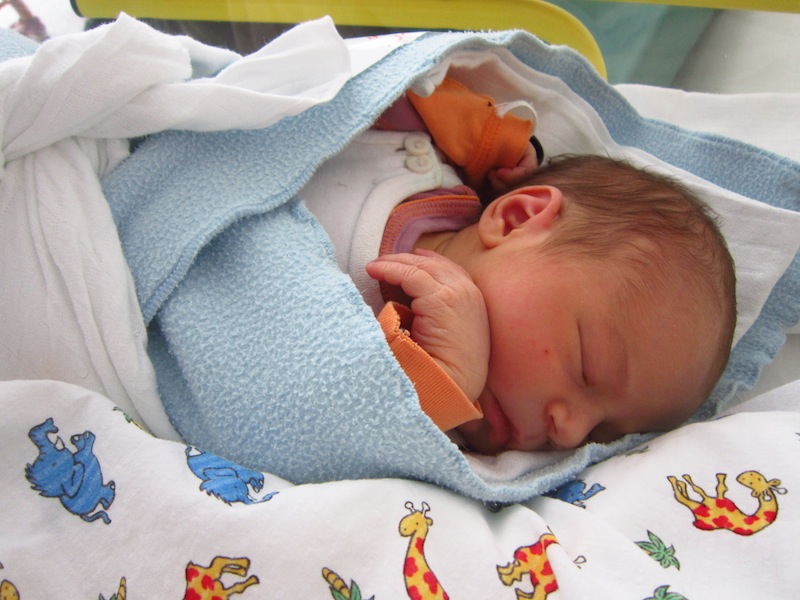
\includegraphics{example.jpg} % requires the graphicx package
%   \caption{example caption}
%   \label{fig:example}
%\end{figure}

%-----<<<<<<<<<<<< NAMES NAD PATHS >>>>>>>>>>>>-----
\def \BookName {Masterer Thesis}
\def \Bookname {Progressive Computation of Global Illumination}
\def \Authors {Author\?: Bc. Zdeněk Glazer}
\def \DatumDP {Prague, 2012}

\def \CVUT {Czech Technical University in Prague}
\def \FEL {Faculty of Electrical Engineering}
\def \DCE {Department of Computer Graphics and Interaction}

\def \cestaFiles {00_Chapters/}
\def \cestaDva {02_Chap2/}
\def \cestaTri {03_Chap3/}
\def \cestaFour{04_SelectedAlgos/}
\def \cestaFive{05_Proposedsolution/}
\def \cestaSix{06_Implementation/}
\def \cestaSeven{07_Results/}
\def \cestaCtyri {04_Concl/}
\def \cestaAP {06_Appendix/}
\def \cestaImg{images/}
%-----<<< --------------------------------- >>>-----

\begin{document}

%-----<<< HEAD >>>-----
\pagestyle{empty}                       %no pagination
\BookHeadDP
\cleardoublepage
%-----<<< ---- >>>-----






%-----<<< ACKNOWLEDGEMENT >>>-----
\input{\cestaFiles Acknow.tex}          %input file
\cleardoublepage
%-----<<< --------------- >>>-----

   %-----<<< DECLARATION >>>-----
\pagestyle{plain}                       %no pagination
\pagenumbering{roman}                   %start roman pagination from 1
\input{\cestaFiles Declar.tex}          %input file
\newpage
\cleardoublepage
%-----<<< ----------- >>>-----

%-----<<< ABSTRACT >>>-----
\input{\cestaFiles Abstract.tex}        %input file
\cleardoublepage
%-----<<< -------- >>>-----


%-----<<< ZAD¡NÕ DIPLOMOV… PR¡CE >>>-----
Vložit zadani prace
\cleardoublepage
%-----<<< ---------------------- >>>-----


   
%-----<<< TABLE OF CONTENTS >>>-----
\setcounter{secnumdepth}{4}             %number of section to 4
\setcounter{tocdepth}{4}                %number of section in table of contents greater then 3
\tableofcontents
\cleardoublepage
%-----<<< ----------------- >>>-----


%-----<<< TABLE OF FIGURES >>>-----
\addcontentsline{toc}{chapter}{List of figures}
\listoffigures
\cleardoublepage
%-----<<< ---------------- >>>-----


%-----<<< TABLE OF TABLES >>>-----
\addcontentsline{toc}{chapter}{List of tables}
\listoftables
\cleardoublepage
%-----<<< --------------- >>>-----


%-----<<< TABLE OF CONTENTS PAGINATION >>>-----
\pagenumbering{arabic}                  %start arabic pagination from 1
%-----<<< ---------------------------- >>>-----


%-----<<< CHAPTERS >>>-----
\hyphenation{Automatica}                %no divide words
\pagestyle{headings}

\chapter{Introduction}
People have always been curious about new forms of visualization and illusion of reality. In the last decade computer generated imagery has reached a state, when majority of the public can't distinguish real photographs from entirely synthesized images. Thanks to this advancements we can enjoy otherwise impossible film shoots, imaginary worlds, visualizations of non existing buildings and much more. All this become possible, because ways how to represent objects and simulate light transport using computer algorithms have been found. The other important factor is ever growing computation power of these devices, which enables us visualize highly detailed datasets with complex materials and challenging lighting scenarios.
\\
\\
Even though many things are possible to simulate and visualize efficiently these days volumetric phenomenons such as clouds, smoke and other optically active medias are still real challenge even for high-end computers. This is all caused by the fact that the data we try to visualized are volumetric and that light passing through can be absorbed, scattered or even emitted in different wavelength (fig aurea borealis). This means that we can no longer assume that visibility of an object can be determined simply by determining if it is hidden behind other object or not.
\\
\\
In terms of feasible render times only direct illumination component can be computed. This approach can give us satisfying results such as those on the figure (fig good rays).  Unfortunately many cool looking effects such as volumetric caustics, which can be seen on the figure (fig lasers) are impossible to get using this approach.
\\
\\
This thesis focuses on methods, which can render anything with physical accuracy and without restrictions on the rendered scene. The other very important bonus of these methods is their progressive nature. In the first passes the corse illumination of the scene is computed and it's progressively refined (fig image getting better). This for example means, that artist defining lighting mood of the visual effect shots can iterate faster. They have got something to show to the director, which results in quick turnarounds and substantial cost and time savings.
\\
\\
Our aim is to implement these progressive Monte Carlo methods in the presence of heterogenous, optically active media and test them on scenes with varying complexity.
\\
\\

%Problem definition tj realistic image synthesis. - done
%
%What is optically active environment and example images. What is challenging in reality immense photon counts, complex light paths and object complexity and dimensionality of the problem. 
%
%Why global illumination - simulace volume caustics (neprime osvetleni muze v osvetlovani hrat i hlavni roli) 
%
%and why progressive methods - artist quick turn arounds with approximated solutions, which show general lighting conditions, quick director approvals. 
%computation is not lost we can continue to render new iterations of the image and increase the fidelity of the image.

% {VULC} vulcano image{images/icevolcano.jpg}
%{LOPT} laser optics {images/laseroptique.jpeg}

\section{Thesis structure}
This Thesis consists of eight main chapters. In the first chapter we have introduced you to the problem. In the second chapter the nifty theoretical details behind realistic image synthesis are exposed and fundamental terms such as BRDF, phase function and rendering equation defined and explained.
\\
\\
The third chapter is an overview of current strategies and algorithms used to visualize the volumetric phenomenons and their pros and cons listed. The fourth chapter leads us to the core of this thesis, the progressive methods of computation the global illumination in the presence of volumetrically active phenomenons.
\\
\\
In the fifth chapter we choose some of the methods mentioned in preceding chapter and further analyze them and propose a way how to and why to use them. In the sixth chapter we present our solution and describe it's internal structure. In the seventh chapter our results and test are shown. And finally eight chapter concludes the information gained and results obtained during this thesis creation.
\\


%\begin{figure}
%   \centering
%   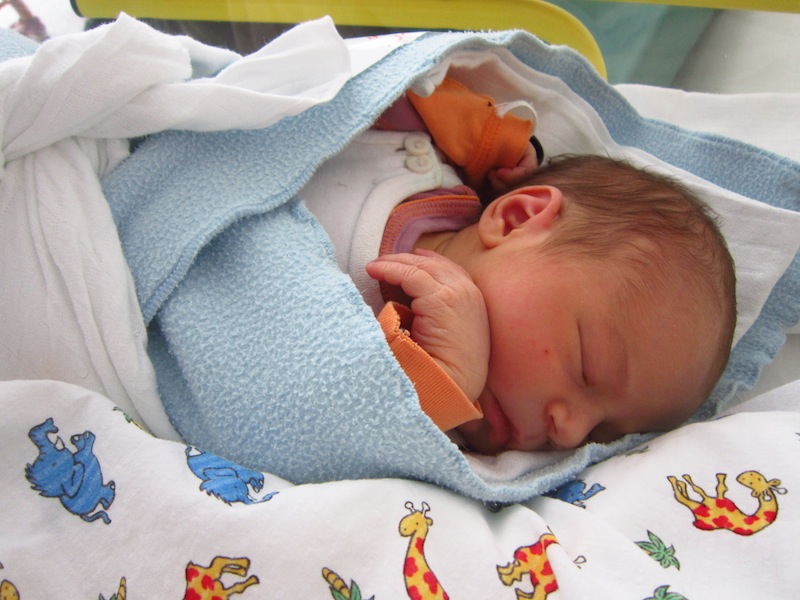
\includegraphics{example.jpg} % requires the graphicx package
%   \caption{example caption}
%   \label{fig:example}
%\end{figure}
%
%   
%Co to je rendering
%Zobrazovaci rovnice distribuce energie v prostoru. 
%
%Co to je raytracing
%paprsek protina geometrii v zakladu 
%
%Jsou stale poupularnejsi progresivni metody renderingu, kdy se obraz pred stale vylepsuje, takze muzem videt nahled velice rychle.
%
%ray tracing se stava poupularnejsi a popularnejsi, mene narocny na nastavovani a fizikalne korektni. Navic sceny jsou slozitejsi a slozitejsi divaci narocnejsi. 
%
%Co to jsou volumetricke efekty a opticky aktivni prostredi
%
%Avsak volumetricke efekty se stale dost casto rasterizujou.
%
%Jak je to náročný a že se stále dost používají aproximační metody (rasterizace, deep shadow maps ) a nemodelují se náročné věci jako radiative transport surface to media volumetric caustics atd. Ani nástroje používané v produkci přímo nepodporuje a nebo jen v podobě náročných fotonových map, je to pomalé , takže artisti nemůžou odladit vse co chteji malo iteraci.



%\section{Podkapitola}
              % input fiel
\input{\cestaDva Chap2.tex} 		% Fundaments of realistic image synthesis
\input{\cestaTri Chap3.tex}		% Common solutions
\input{\cestaFour Chap4.tex}		% Consistant progressive methods
\input{\cestaFive Chap5.tex}		% Proposed solutions
\input{\cestaSix Chap6.tex}		% Implementation
\input{\cestaSeven Chap7.tex}		% Results

\input{\cestaCtyri Concl.tex}		% Conclusion
%-----<<< -------- >>>-----


%-----<<< REFERENCES >>>-----
%\begin{thebibliography}{xx}

% ======== reference k progressive beam mappingu atd =====
@article{novak12vbls,
    author = {Jan Nov{\'a}k and Derek Nowrouzezahrai and Carsten Dachsbacher and Wojciech Jarosz},
    title = {Progressive Virtual Beam Lights},
    journal = {Computer Graphics Forum (Proceedings of EGSR 2012)},
    volume = {31},
    number = {4},
    year = {2012},
    month = jun,
    keywords = {photon beams, photon mapping, final gather, participating media, VPL, virtual point lights, VSL, virtual spherical lights, indirect illumination, weak singularity}
}

@article{jarosz11comprehensive,
    author = {Wojciech Jarosz and Derek Nowrouzezahrai and Iman Sadeghi and Henrik Wann Jensen},
    title = {A Comprehensive Theory of Volumetric Radiance Estimation Using Photon Points and Beams},
    journal = {ACM Transactions on Graphics (Presented at ACM SIGGRAPH 2011)},
    volume = {30},
    number = {1},
    year = {2011},
    month = jan,
    pages = {5:1--5:19},
    keywords = {photon beams, photon mapping, beam radiance estimate, density estimation, participating media}
}

@article{novak12vrls,
    author = {Jan Nov{\'a}k and Derek Nowrouzezahrai and Carsten Dachsbacher and Wojciech Jarosz},
    title = {Virtual Ray Lights for Rendering Scenes with Participating Media},
    journal = {ACM Transactions on Graphics (Proceedings of ACM SIGGRAPH 2012)},
    volume = {31},
    number = {4},
    year = {2012},
    month = jul,
    keywords = {photon beams, photon mapping, final gather, participating media, VPL, virtual point lights, indirect illumination, weak singularity, unbiased}
}

@article{jarosz11progressive,
    author = {Wojciech Jarosz and Derek Nowrouzezahrai and Robert Thomas and Peter-Pike Sloan and Matthias Zwicker},
    title = {Progressive Photon Beams},
    journal = {ACM Transactions on Graphics (Proceedings of ACM SIGGRAPH Asia 2011)},
    volume = {30},
    number = {6},
    year = {2011},
    month = dec
}

@article{jarosz08beam,
    author = {Wojciech Jarosz and Matthias Zwicker and Henrik Wann Jensen},
    title = {The Beam Radiance Estimate for Volumetric Photon Mapping},
    journal = {Computer Graphics Forum (Proceedings of Eurographics 2008)},
    volume = {27},
    number = {2},
    year = {2008},
    month = apr,
    pages = {557--566}
}

% ========End of: reference k progressive beam mappingu atd =====



% ======== reference k progressive photon mappingu

%========End of:  reference k progressive photon mappingu

%======== neco k volume renderingu sampling + deep shadow mapping, furier maps atd.

%======== End of:  neco k volume renderingu sampling + deep shadow mapping, furier maps atd.



\end{thebibliography}



\bibliographystyle{alphaurl}
\bibliography{mybibliography}

%\bibliographystyle{Styles/Skripta}
%\bibliography{Styles/Refer}                   %references from BIBTEX
\addcontentsline{toc}{chapter}{Literatura}
%-----<<< ---------- >>>-----

%-----<<< APPENDIXS >>>-----
\cleardoublepage
\def\appendixname{Appendinx}
\pagenumbering{Roman}                   %start arabic pagination from 1
\begin{appendix}
\input{\cestaAP Appen1.tex}             %input file
\input{\cestaAP Appen2.tex}             %input file
%\input{\cestaAP Appen3.tex}             %input file
\end{appendix}
%-----<<< --------- >>>-----

   
   
  \end{document}